\documentclass[fleqn]{article}[12pt]

\usepackage{amsmath}
\usepackage{amssymb}
\usepackage{pgfplots}
\usepackage[margin=1in]{geometry}
\usepackage{fancyhdr}
\usepackage{lastpage}
\usepackage{siunitx}
\usepackage{amsthm}


\setlength\parindent{0pt}

\cfoot{\thepage \hspace{1pt} / \pageref{LastPage}}
\newcommand{\integral}[4]{\int_#1^#2 \! #3 \, \mathrm{d}#4}
\newcommand{\dif}{\mathrm{d}}
\newcommand{\diracraw}{\left(\int_{-\infty}^{\infty} e^{i2\pi (f - \bar f)}\, dt\right)}
\usepackage{caption}
\captionsetup{justification=raggedright,singlelinecheck=false}
\DeclareMathOperator{\Imag}{Im}


\DeclareSIUnit\year{yr}

\pgfplotsset{compat=1.14}

\newcommand{\M}{\mathbb{M}}
\newcommand{\W}{\mathbb{W}}
\newcommand{\R}{\mathbb{R}}


\begin{document}
    \begin{tabular}{l}
        ID \#33 \\
        Problem Set 4 \\
        Physics 202 \\
        \today
    \end{tabular}

\begin{enumerate}
    \item \begin{enumerate}
        \item
        \begin{equation*}
            \Delta t = \Delta t_0 \frac{1}{\sqrt{1-(u/c)^2}} = \SI{100}{\nano\s}\frac{1}{\sqrt{1-(0.96c)^2}} = \SI{357}{\nano\s}
        \end{equation*}
        \item
        \begin{equation*}
            d = v \Delta t = (0.96c)\SI{357}{\nano\second} = \SI{102.82}{\m}
        \end{equation*}
        \item
        \begin{equation*}
            d_0 = v \Delta t_0 = (0.96c)\SI{100}{\nano\second} = \SI{28.8}{\m}
        \end{equation*}
    \end{enumerate}

    \item \begin{enumerate}
        \item Let the period of the light given off by the source be $\Delta t$, and $A$ and $B$ be successive points where the wave reaches a peak. Assuming these paths are near-identical, the difference in path lengths is
        \begin{equation*}
            v \Delta t \cos(\theta)
        \end{equation*}
        since $v \Delta t$ is the distance traveled by the source in that time, and $\cos(\theta)$ is the component of that velocity going towards $Q$. Since the time between peaks from a stationary source is $c\Delta t$, the distance between peaks is
        \begin{equation*}
            \Delta t_0' = (1-\beta\cos(\theta))\Delta t c
        \end{equation*}
        However, we also need to factor in the length dilation due to relativistic speeds. This gives that
        \begin{equation*}
            \frac{f_{obs}}{f_{sce}} = \frac{1}{(1-\beta\cos(\theta))\Delta t c} \frac{\Delta t c}{\gamma} \implies f_{obs} = \frac{f_{sce}}{(1-\beta \cos(\theta))\gamma}
        \end{equation*}

        \item When the source is approaching head-on, $\theta=0$. Using the equation from above,
        \begin{equation*}
            f_{obs} = \frac{f_{sce}}{(1-\beta \cos(0))\gamma} = \frac{f_{sce}}{(1-\beta)\gamma}
        \end{equation*}
        which matches what we expect for an approaching source. When the source is receding directly away, $\theta=\pi$, and
        \begin{equation*}
            f_{obs} = \frac{f_{sce}}{(1-\beta \cos(\pi))\gamma} = f_{obs} = \frac{f_{sce}}{(1+\beta)\gamma}
        \end{equation*}
        which is again what we expected.

        \item The frequency observed on the detector is
        \begin{equation*}
            f_{obs} = \frac{f_{sce}}{(1-\beta \cos(\pi/2\pm\pi/4))\gamma} = \frac{\SI{250e18}{\hertz}}{(1\mp0.3/\sqrt{2})(1.048)} = \SI{302e18}{\hertz}, \SI{196e18}{\hertz}
        \end{equation*}

        With detectors at $\SI{135}{\degree}$, the readings would be identical, since $\theta$ would simply be negative, and $\cos(-\theta) = \cos(\theta)$. With detectors at $\SI{90}{\degree}$,
        \begin{equation*}
            f_{obs} = \frac{f_{sce}}{(1\pm\beta)\gamma} = \SI{341e18}{\hertz}, \SI{183e18}{\hertz}
        \end{equation*}

    \end{enumerate}

    \item \begin{enumerate}
        \item This is calculated using the Doppler shift equation:
        \begin{equation*}
            (\SI{1}{\year^{-1}})\sqrt{\frac{1-0.6}{1+0.6}} = \SI{0.5}{\year^{-1}}
        \end{equation*}

        \item
        \begin{equation*}
            (\SI{1}{\year^{-1}})\sqrt{\frac{1+0.6}{1-0.6}} = \SI{2}{\year^{-1}}
        \end{equation*}
        The reason these results are the same as found for Casper's signals from Amelia is because, from Amelia's perspective, Casper is going away from her at $0.6c$, and then returning---same as her travels appear to Casper.

        \item Amelia measured the 20-year journey to take
        \begin{equation*}
            \SI{20}{\year} = \Delta t \frac{1}{\sqrt{1-(0.6c)^2}} \implies \Delta t = \SI{16}{year}
        \end{equation*}
        Therefore, Casper will receive 16 signals, since Amelia measured the passing of 16 years.
    \end{enumerate}

    \item
    \begin{tikzpicture}[remember picture, overlay,shift={(current page.north west)}]
  \draw[very thin, blue!10,step=2mm]
  (current page.south west) grid (current page.north east);
  \draw[very thin, red!20,step=1cm]
  (current page.south west) grid (current page.north east);
\end{tikzpicture}
\end{enumerate}


\end{document}
